%Technical Review template made by Jeroen Hanselman for MaRDI (Mathematical Research Data Initiative)
%
% The template used for this technical review was adapted from the template made by Timmy Chan on https://github.com/TimmyChan 

%====================
% Packages and initialization
%====================
\documentclass[10pt]{article}
\usepackage[utf8]{inputenc}
\usepackage{graphicx}
\usepackage{pifont,xcolor}
\usepackage{amssymb}
\usepackage{TLCresume}
\usepackage{tikz}
\usepackage{parallel,enumitem}

%====================
% Colors and commands useful for the review
%====================
\definecolor{mardiblue}{RGB}{4,91,167}
\definecolor{mardiorange}{RGB}{208,102,49}

\newcommand{\mplus}[1][mardiblue]{
  \begingroup\leavevmode\color{#1}
  \setlength{\unitlength}{0.8em}
  \linethickness{.25em}
  \begin{picture}(1,1)
  \put(0,0.5){\line(1,0){1}}
  \put(0.5,0){\line(0,1){1}}
  \end{picture}
  \hspace{0.2em}
  \endgroup
}

\newcommand{\mminus}[1][mardiorange]{
  \begingroup\leavevmode\color{#1}
  \setlength{\unitlength}{0.8em}
  \linethickness{.25em}
  \begin{picture}(1,1)
  \put(0,0.5){\line(1,0){1}}
  \end{picture}
  \hspace{0.2em}
  \endgroup
}

\makeatletter
\newcommand*{\radiobutton}{
  \@ifstar{\@radiobutton0}{\@radiobutton1}
}
\newcommand*{\@radiobutton}[1]{
  \begin{tikzpicture}
    \pgfmathsetlengthmacro\radius{height("X")/2}
    \draw[radius=\radius] circle;
    \ifcase#1 \fill[radius=.6*\radius] circle;\fi
  \end{tikzpicture}
}
\makeatother

%====================
% Title of paper and authors
%====================
\def\titleofpaper{Algorithm to compute the number of carrots needed to complete a proof} 
\def\authors{Jeroen Hanselman and Mardi the Math bunny}

%====================
% Review Header
%====================

\RequirePackage{fancyhdr}
\fancypagestyle{fancy}{%
\fancyhf{}
\lhead{



\textbf{Title: }\titleofpaper\\
\textbf{Author(s): }\authors  \\
\textbf{} \\
\textbf{Date: }\today\\ 
	    } 
	\chead{%
	    \centering {\huge \textbf{Technical review}} \\ %
	    }%
	    
\rhead{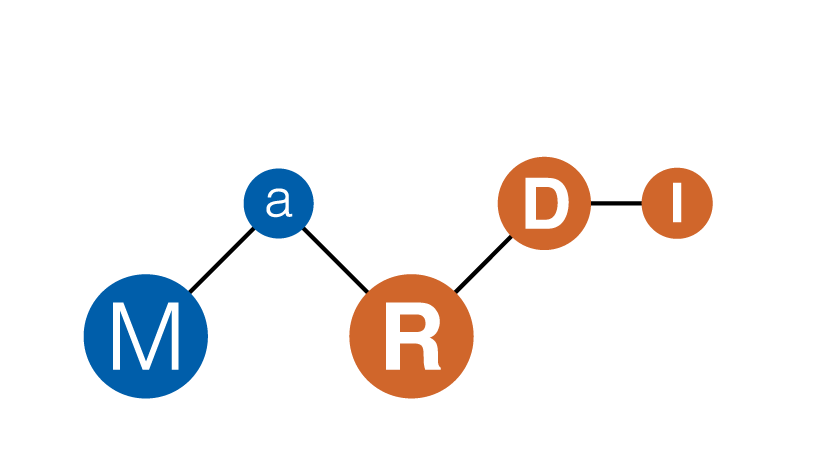
\includegraphics[scale=0.7]{Mardi.png}}
\renewcommand{\headrulewidth}{2pt}% 2pt header rule
\renewcommand{\headrule}{}
}
\pagestyle{fancy}

\setlength{\headheight}{150pt}
\setlength{\headsep}{5pt}

\begin{document}


%====================
% Sections of the review
%====================
\section{Basic Info}
%====================
% Basic Info
%====================
% Here you can indicate which files were included with the paper.
\begin{minipage}{0.30\textwidth}
\noindent\parbox[t]{1.2in}{\raggedright%
\vspace{0.5em}
\textbf{Files provided}

\begin{itemize}[topsep=0pt,itemsep=-2pt,leftmargin=13pt]
\item[$\boxtimes$] Source Code
\item[$\square$] Notebook
\item[$\square$]  Examples
\item[$\square$] Docker file/VM
\end{itemize}

\vspace{0.5em}
}%
\parbox[t]{1.2in}{\raggedright%
\vspace{1em}
\begin{itemize}[topsep=6pt,itemsep=-2pt,leftmargin=13pt]
\item[$\boxtimes$]  Documentation
\item[$\square$]  Computed data
\item[$\square$] Files that verify computed data
\end{itemize}
\vspace{0.5em}
}
\end{minipage}%
\hfill
%
% Here you can list all the information about what software and hardware was used to perform the review, as well as which version of the code was reviewed.
%
\begin{minipage}{0.6\textwidth}
\begin{tabular}[t]{p{13em} p{1em} p{17em}}
\textbf{Programming languages:} & &  N/A \\
\textbf{Standard software used: }& &  Magma V2.27-8   \\
\textbf{System specs used for review :}& &  Ubuntu 22.04.1 with Intel i7-7700 processor, 4 cores @ 3.60GHz, 32GB RAM \\
\textbf{Version reviewed (Magma):}& &  No version numbering. Files reviewed were last changed on the 11th of March 2024\\
\textbf{Downloaded from (Magma): }& &   \url{https://github.com/fakegithub/MathBunnyMadness} \\

\end{tabular}
\end{minipage}%

\section{Importance of software in the paper}
%====================
% Importance
%====================
% Here you can indicate the code plays in the paper. Depending on what this is the focus of the review might be a bit different.  

The repository contains the implementation of the algorithms and the results of the computations described in the paper.\\


\section{Reproducibility (Installation)}
%====================
% Installation
%====================
% Here everything that has to with with installing the software can be written. Was the code available? Are other people allowed to reuse it for their own research, i.e. does the license allow for it? Does the repository have a proper readme allowing you to understand what is what? Are there proper installation instructions? Was it easy to install the software?


\begin{tabular}[t]{p{15 em} p{1em} p{35em}} 
\textbf{License:}  & & \mminus No license found\\
\textbf{Availability: }& & \mplus The files were uploaded to GitHub \\
\textbf{Readme:} & & \mplus The repository contains a Readme explaining the contents of the Github. \\
\textbf{Installation:} & & \mplus Straightforward. \\
\end{tabular}


\section{Installation steps taken}
%====================
% Installation Steps
%====================
% Here you describe what steps you took to try to install the software. Especially helpful for the authors when you fail to install the software because they can then see what you tried to do.
\textbf{Magma Code:}
\begin{itemize}
\item Cloned \verb|https://github.com/MaRDItheMathbunny/MaRDICode| from GitHub
\end{itemize}

\section{Reproducibility (Records of setup)}
%====================
% Recordsd of setup
%====================
% Here you write down whether the authors wrote down the specs of their system or OS that they used to produce their results. This is more important when the authors have code that takes a long time to run or when they compare their algorithm with other algorithms.

\begin{tabular}[t]{p{15 em} p{1em} p{35em}}
\textbf{Specification of CPU:}& & \mminus Did not find what CPU was used. \\
\textbf{Specification of Memory:}& & \mminus Did not find the amount of memory used. \\

\textbf{Specification of OS/software used:}& & \mminus Did not find which Magma version was used. \\
\textbf{References and citation: }& & \mplus Magma is cited. The other packages the software builds on or depends on are properly cited.\\
\end{tabular}

\section{Reproducibility (Running the code)}
%====================
% Reproducibility
%====================
% Here you describe whether you were able to run the code that was provided. You can furthermore mention any errors that showed up.

\begin{tabular}[t]{p{15 em} p{1em} p{35em}}

\textbf{Magma Code:} & & \mplus The code seems to run fine. It does give a small error however: \begin{verbatim}
In file "Carrot.m", line 587, column 9:
>> bunny := [ 0, 0, 0];
\end{verbatim}
\\

\end{tabular}

\section{Correctness and Reliability}
%====================
% Correctness and Reliability
%====================
% In this section you can indicate how convinced you are that the code does what is claimed in the paper. Thinks that might make results more convincing are, for example, trying out different inputs, test files written by the authos or multiple implementations in different systems. But these are not strictly necessary. This section is mostly about if the output coincides with what was claimed and if the algorithms seem to be doing the correct thing.

\begin{tabular}[t]{p{15 em} p{1em} p{35em}}
\textbf{Recalculating the examples:} & & \mminus I find it a bit hard to check whether the code produces the same results as what the authors got. There are a lot of files in the Github and it was unclear to me what files I should look at.
\end{tabular}

\section{Readability}
%====================
% Readability
%====================
% In this section you describe whether the code looks easy to read. Are variable names chosen in a meaningful way? Is the code properly indented?, etc.
\begin{tabular}[t]{p{15 em} p{1em} p{35em}}
\textbf{Annotation :} & & \mplus The code is clearly annotated. \\
\textbf{Indentation and formatting:} & & \mplus   Consistent.\\
\textbf{Naming of variables : }& & \mplus Consistent, meaningful and distinctive. \\
\end{tabular}
 
\section{Comments}
%====================
% Comments
%====================
% Here you can list any comments you would like to pass on to the authors or any specific details about the review that did not fit anywhere else.
None.


\end{document}
